\documentclass[10pt,a4paper]{article}

%% packages
\usepackage{color}
\usepackage{pgf}
\usepackage[margin=1in]{geometry}
\usepackage[normalem]{ulem}
\usepackage{cite}
\usepackage{natbib}
\usepackage{authblk}
\usepackage{listings}
\usepackage{color}
\usepackage[colorlinks=true,
            linkcolor=red,
            urlcolor=blue,
            citecolor=gray]{hyperref}
 
\definecolor{dkgreen}{rgb}{0,0.6,0}
\definecolor{gray}{rgb}{0.5,0.5,0.5}
\definecolor{mauve}{rgb}{0.58,0,0.82}
           
\lstset{frame=tb,
  language=bash,
  frame=none,
  aboveskip=3mm,
  belowskip=3mm,
  showstringspaces=false,
  columns=flexible,
  basicstyle={\small\ttfamily},
  numbers=none,
  numberstyle=\tiny\color{gray},
  keywordstyle=\color{blue},
  commentstyle=\color{dkgreen},
  stringstyle=\color{mauve},
  breaklines=true,
  breakatwhitespace=true,
  tabsize=3
}

\usepackage[colorinlistoftodos]{todonotes}
\definecolor{flame}{rgb}{0.89, 0.35, 0.13}
%\setlength{\marginparwidth}{1.5cm}
\newcommand{\jri}[1]{\todo[size=\scriptsize, color=flame]{#1}}
            
\newcommand{\X}{\textcolor{red}{\bf X}}


\title{More than one Author with different Affiliations}
\author[1,$\dag$]{Arun Durvasula}
\author[2,$\dag$]{Paul J. Hoffman}
\author[1]{Tyler V. Kent}
\author[2]{Chaochih Liu}
\author[2]{Thomas J. Y. Kono}
\author[2]{Peter L. Morrell}
\author[1,3,*]{Jeffrey Ross-Ibarra}
\affil[1]{Department of Plant Sciences, University of California, Davis, CA 95616}
\affil[2]{Department of Agronomy and Plant Genetics, University of Minnesota, St. Paul, MN 55108}
\affil[3]{Center for Population Biology and Genome Center, University of California, Davis, CA 95616}
\affil[$\dag$]{These authors contributed equally.}
\affil[*]{email: rossibarra@ucdavis.edu}


\renewcommand\Authands{ and }

\begin{document}

\title{ANGSD-wrapper: utilities for analyzing next generation sequencing data}
\maketitle

\begin{abstract}
High throughput sequencing has changed many aspects of population genetics, molecular ecology, and related fields, affecting both experimental design and data analysis.
The software package ANGSD allows users to perform a number of population genetic analyses on high-throughput sequencing data. 
The package is specifically designed to produce more accurate results for samples with low sequencing depth and makes use of full genome data while handling a wide array of sampling and experimental designs.
Here we present ANGSD-wrapper, a user-friendly interface for running ANGSD and visualizing results.
ANGSD-wrapper includes a number of 'wrapper' scripts that facilitate configuration and execution of multi-step analyses and provides interactive graphing of ANGSD results to enhance data exploration.
We demonstrate the usefulness of ANGSD-wrapper by analyzing resequencing data from populations of wild and domesticated \textit{Zea}. 
ANGSD-wrapper is freely available from \url{https://github.com/mojaveazure/angsd-wrapper}.
\end{abstract}

\section*{Introduction}

High throughput sequencing has revolutionized evolutionary genetics, allowing researchers to quickly assay large numbers of individuals or survey fine-scale patterns of variation along the genome.  
Application of these methods has led to changes in both experimental design and data analysis \citep{ekblom2011applications}.
Many of the popular software packages used by researchers \citep[see][]{excoffier2006computer}  were not designed to handle these novel data types or efficiently analyze the large volumes of data now being generated. 
In particular, short read sequencing has brought new challenges, including highly variable coverage, missing data, and high per-nucleotide error rates.

A number of tools have recently been published to handle high throughput sequencing data \citep{garrigan2013popbam, purcell2007plink, danecek2011variant, hutter2006genome}, but the majority of these either make limiting assumptions about the data (e.g., all sites have been sequenced, all genomes are haploid, sequencing is to sufficient depth, all individuals are outcrossing) or are specialized tools offering a narrow set of analysis options. 
Korneliussen et al. \citep{korneliussen2014angsd} recently published the software package ANGSD, which enables users to flexibly perform a large number of common population genetic analyses, including diversity statistics, admixture analysis including Patterson's D statistic \citep{Durand:2011jd}, site frequency spectrum estimation \citep{pmid22911679}, and neutrality test statistics \citep{korneliussen_calculation_2013}. %\jri{are all these within ANGSD or are some ngsPopgen?} all are in ANGSD
One of the most important features of ANGSD is that most analyses are performed directly on genotype likelihoods, freeing users from the requirement of calling variants or genotypes and permitting analysis of low-coverage data or sequences with large amounts of missing data. 

Here we present ANGSD-wrapper, a user-friendly interface to ANGSD. 
ANGSD-wrapper takes the form of a set of configuration files and 'wrapper' scripts (Figure \ref{fig:supp2}) that streamline the execution of multi-step pipelines inherent in ANGSD as well as pipelines involving related programs such as ngsPopGen, ngsF\citep{vieira2013estimating}, and ngsAdmix \citep{pmid24026093}.
Because the large volume of data associated with high throughput sequence analysis is often difficult to explore by hand, ANGSD-wrapper also provides a suite of interactive visualization tools to plot results and explore patterns at multiple scales.  
We demonstrate some of the analyses possible using ANGSD-wrapper using low-coverage whole-genome data from domesticated maize and two related wild teosinte subspecies. 
ANGSD-wrapper is freely available from \url{https://github.com/mojaveazure/angsd-wrapper}.

\section*{Methods}
ANGSD-wrapper is a set of configuration files and scripts written in the Bash UNIX shell.  
The scripts can be run either on a standalone computer with a UNIX terminal, or on computing clusters where they can be submitted to a queuing system such as SGE \citep{Microsystems):2001:SGE:560889.792378}, Slurm \citep{Jette02slurm:simple} or TORQUE \citep{Staples:2006:TRM:1188455.1188464}.  
An installation of the statistical software R \citep{Rcitation} is required to make use of the visualization tools incorporated in ANGSD-wrapper.  
The visualization portion of ANGSD-wrapper also requires installation of the R packages shiny \citep{shiny}, genomeIntervals \citep{genomeIntervals}, and ape \citep{APE}.


\begin{table}
\begin{center}
    \begin{tabular}{ | p{5cm} | p{5cm} |}
    \hline
    \textbf{Methods Implemented} & \textbf{Interactive Graphing} \\ \hline \hline
    Patterson's D (ABBA-BABA) & Yes \\ \hline
    Admixture & Yes  \\ \hline
    Ancestral Sequence & No \\ \hline
    Genotype Likelihoods & No \\ \hline
    Inbreeding Coefficients & No \\ \hline
    PCA & Yes \\ \hline
    Site Frequency Spectrum & Yes \\ \hline
    Diversity Statistics ($\theta_w$, $\theta_\pi$, Fu and Li's $\theta$, Fay's $\theta$)   & Yes \\ \hline
    Neutrality Test Statistics (Tajima's D, Fu and Li's D, Fu and Li's F,  Fay and Wu's H, Zeng's E ) & Yes \\ \hline
    Fst & Yes \\ \hline
    \end{tabular}
    \caption{Table of methods implemented in ANGSD-wrapper}
    \label{tab:methods}
    \end{center}
\end{table}
%\jri{in table: list diversity statistics in parentheses. what about Fst?} done. and added Neutrality test stats

ANGSD-wrapper is divided into scripts associated with analytical approaches implemented in ANGSD and associated software. 
ANGSD-wrapper provides a common configuration file, common.conf, which  holds variables that are likely to remain constant across analyses, including identifiers for chromosomal regions and the paths to project directories.
In ANGSD-wrapper, each method is self-contained in a shell script which uses information from the common configuration file and a method-specific configuration file. 
Each analysis is run using a simple command:

\begin{lstlisting}
$ angsd-wrapper <method> <configuration_file>
\end{lstlisting}

Analyses supported by ANGSD-wrapper are shown in table \ref{tab:methods}, and a detailed flowchart of each of these workflows is shown in Figure \ref{fig:supp2}, and additional details, documentation, a tutorial, and a wiki can be found on the GitHub page: \url{https://github.com/mojaveazure/angsd-wrapper/wiki}.

The visualization software included with ANGSD-wrapper is contained within it's own directory called shinyGraphing.
This application must be started in R and can be accessed locally from a web browser. This software provides a graphical user interface (GUI) to quickly and interactively plot results obtained from ANGSD-wrapper.  
Each tab in the GUI contains plots for different ANGSD methods.

In order to use the plotting software, the user navigates to the desired tab and uploads the appropriate file of results. 
The Shiny server automatically parses ANGSD output files and creates the resulting plot(s) (Figure \ref{fig:theta}), which can be saved using the browser's built in image saving capabilities. % \jri{add genes from gff. i don't think it's Mb 1-10, pls check. if so, is x-axis wrong?} done

\begin{figure}
\centering
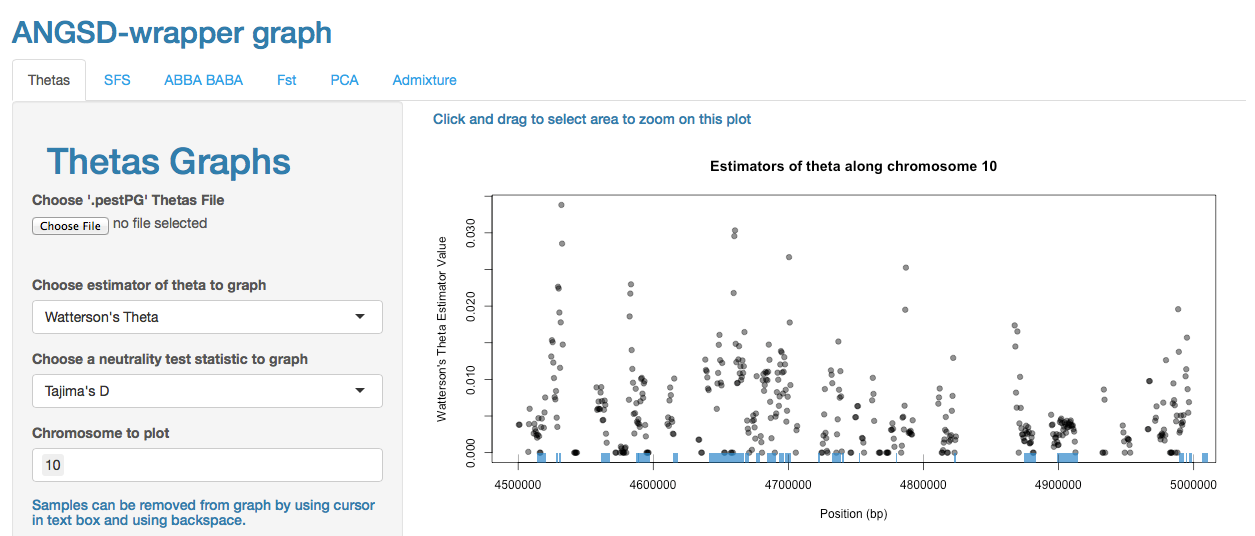
\includegraphics[width=130mm]{figures/fig1.png}
\caption{A visualization of Watterson's $\theta$ estimated by ANGSD across a 1.5 megabase region of chromosome 10 in {\it Zea mays} spp. {\it mays} using ANGSD-wrapper. Blue boxes indicate genic regions provided by a GFF annotation. \label{fig:theta} }
\end{figure}

\section*{Example data}
% \jri{show k=2 and k=3 for adxmxture in supp.} done
\begin{figure}
\centering
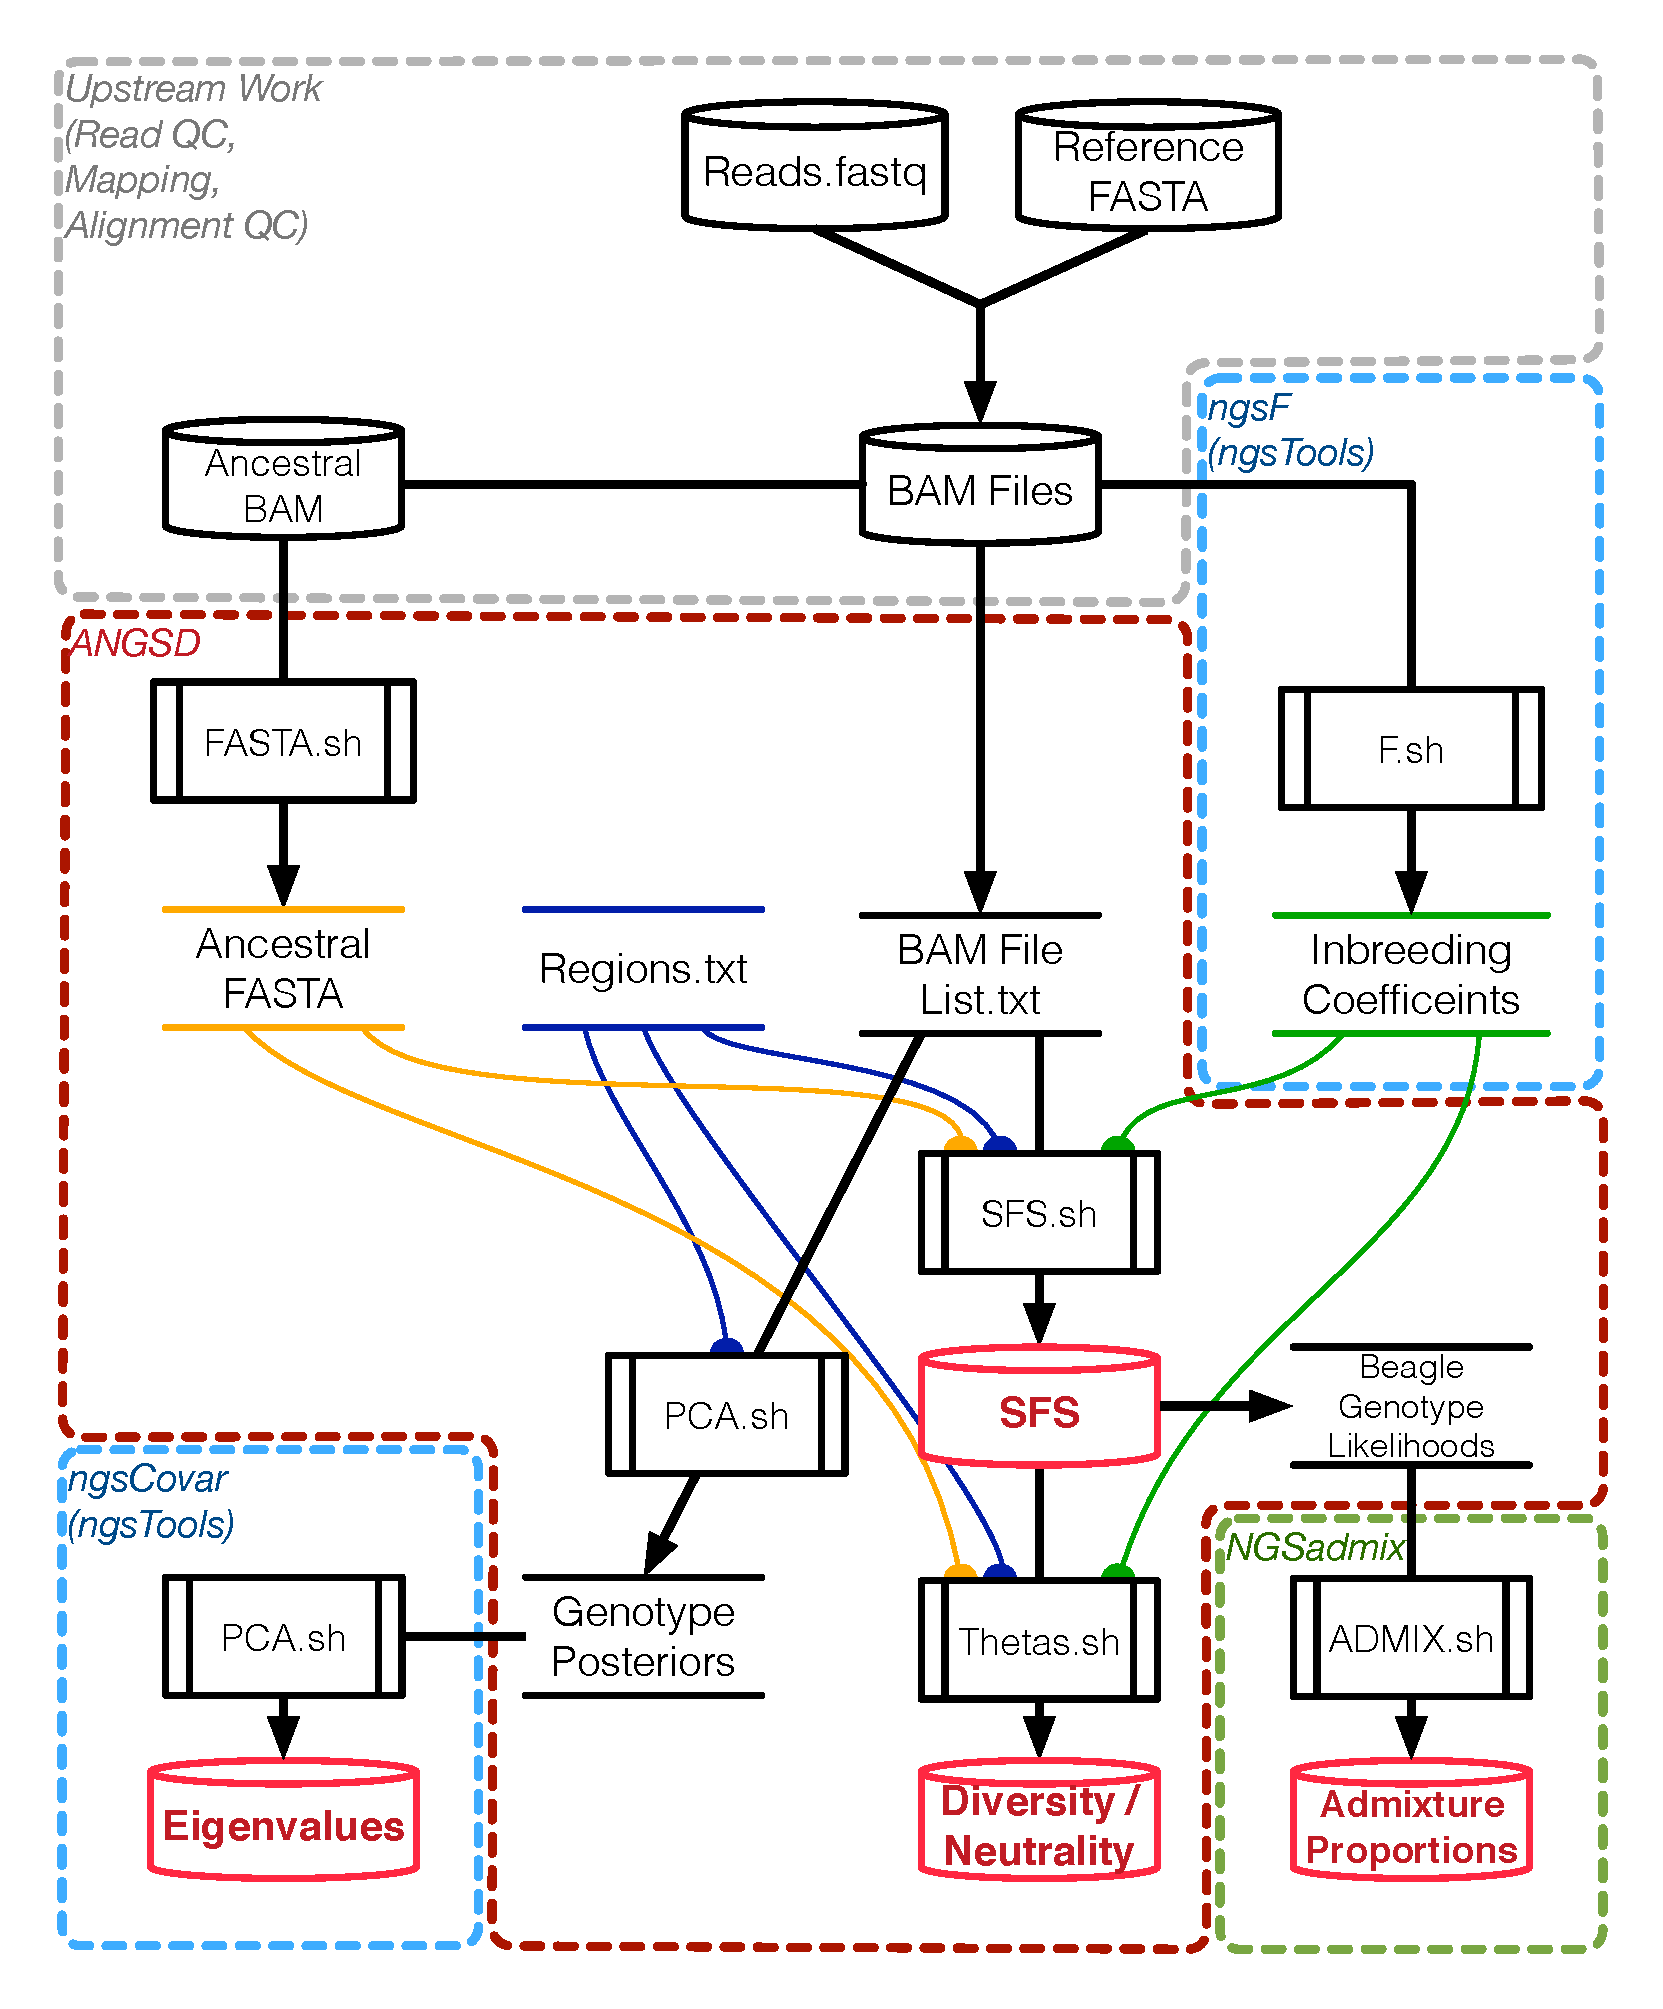
\includegraphics[width=\linewidth]{figures/MainTextWorkflow.pdf}
\caption{Example analysis workflow diagram.}
\label{fig:workflow}
\end{figure}

\begin{figure}
\centering
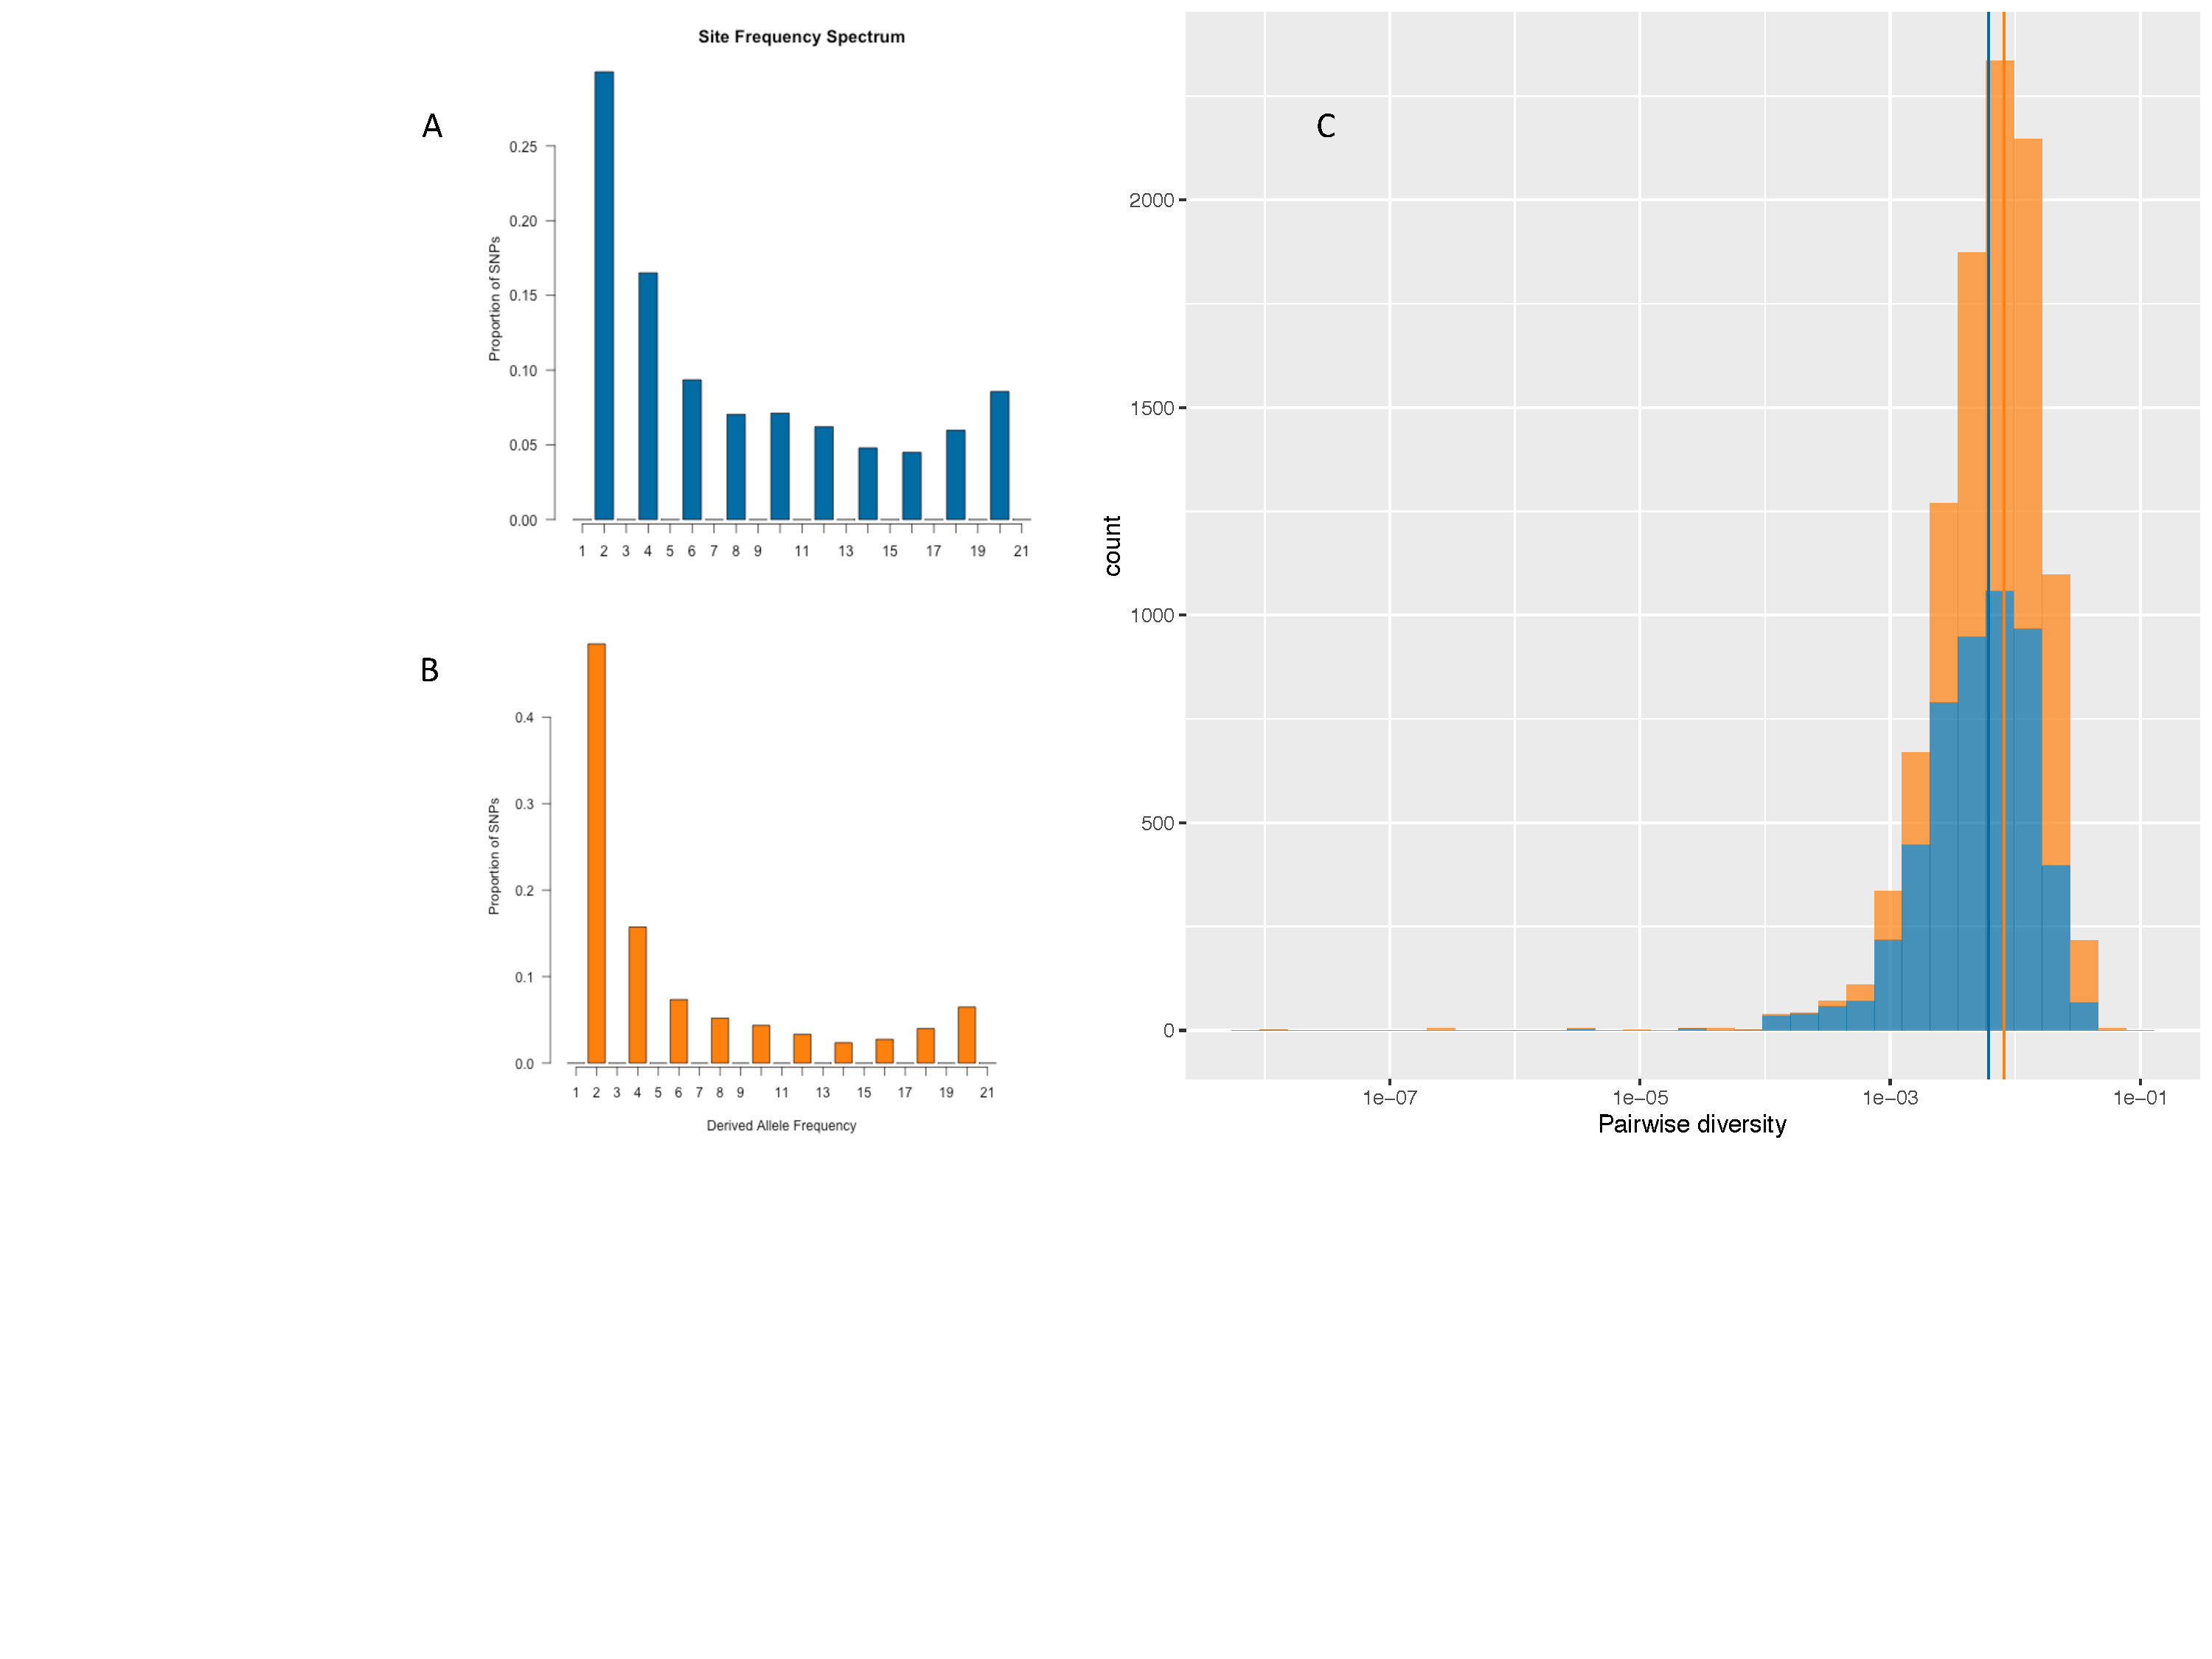
\includegraphics[width=\linewidth]{figures/figure3big.pdf}
\caption{Summary statistics for {\it Zea mays}. Site frequency spectra for A. maize and B. teosinte. C. distribution of pairwise differences for maize (blue) and teosinte (orange). Pairwise diversity results are visualized separately from the interactive graphics and colors were added to A and B using a custom script.}
\label{fig:figure3}
\end{figure}

\begin{figure}
\centering
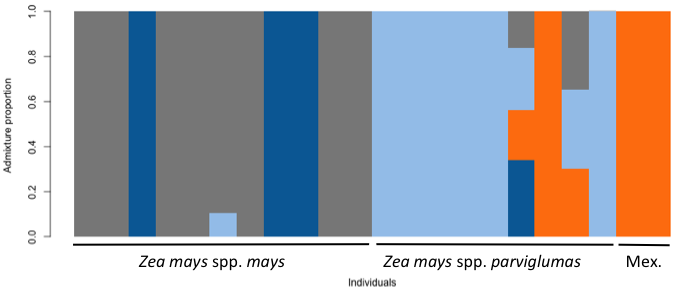
\includegraphics[width=\linewidth]{figures/mt4labeled.png}
\caption{Admixture analysis for {\it Zea mays} spp. {\it mays}, {\it Zea mays} spp. {\it parviglumas}, and {\it Zea mays} spp. {mexicana} (\texit{mex}) with K=4 source populations. For a list of samples see Table \ref{tab:samples}. }
\label{fig:admixture}
\end{figure}

% \jri{change Mex to mex and make italics in figure axis} done

As a demonstration of analyses in ANGSD-wrapper, we explore patterns of diversity in a single genomic region of a subset of domesticated maize and wild teosinte. We used resequenced samples from the HapMap2 project  and calculated summary statistics using a 10 megabase region on chromosome 10 \citep{chia2012maize} .\jri{include download link.}

We first use the SFS method to estimate the site frequency spectrum (SFS) of both maize and its wild progenitor \textit{Zea mays} ssp. \textit{parviglumis}, assuming an inbreeding coefficient of $F=1$ since these are all highly inbred samples. %\jri{do we worry that fig. 3 not graphs directly from A-W?} % noted this in the figure legend, SFSes are basically from AW, just colors changed. In the future should we add color picker for SFS?

Consistent with previous results \citep{hufford2012comparative}, we show that the maize SFS is skewed towards more intermediate-frequency variants (Figure \ref{fig:figure3}A-B), likely a result of the bottleneck associated with maize domestication \citep{Beissinger031666}.
We find further evidence of the effect of domestication using the Thetas method, revealing lower levels overall levels of diversity in maize (Figure \ref{fig:figure3}C). These results use Tripsacum as an ancestral sequence, which was generated using the Ancestral Sequence method in ANGSD-wrapper. %\jri{fill in \X's with which A-W script we used. probably need to modify this to mention Tripsacum and generation of the ancestral seq. and which A-W script we used for that.} done
Using the 2DSFS method, which includes an $F_{ST}$ calculation, we then scan our example region for windows with elevated differentiation between maize and teosinte. 
The mean $F_{ST}$ in this region is 0.013, which is an order of magnitude lower than the genome-wide reported value of 0.11 \citep{hufford2012comparative}.   
The \X windows in the 1\% tail of highest $F_{ST}$ values include genes several genes identified as potential targets of selection during domestication in \citep{hufford2012comparative} \jri{see supp tables in Huff. make supp. table of genes in top 1\%. sorry to add, but this is cool \& demonstrates more stuff A-W can do. don't need a graph}

Finally, we include two samples of the related wild teosinte \textit{Zea mays} ssp. {mexicana} to assess evidence for admixture.  
Figure \ref{fig:admixture} identifies structure within the domesticated maize separating three high-latitude temperate landraces from the other tropical accessions. 
We find no evidence of admixture between these lowland maize samples and  ssp. {mexicana}, consistent with an independent analysis using SNP genotyping \citep{hufford2013genomic}.
\textit{Zea mays} ssp. {mexicana} clusters into its own group, along with a single accession of ssp. {parviglumis} collected from region in which many teosinte populations appear to be the result of admixture between the two subspecies \citep{fang2012megabase}.  A single  ssp. {parviglumis} accession from the Northern extent of the range does not appear to be well-classified with these data, likely due to our relatively limited geographic and genomic sampling.

\section*{Conclusions}
Our software ANGSD-wrapper provides an intuitive and easy-to-use interface to employ the powerful and flexible suite of population genetic analyses developed in ANGSD \citep{korneliussen2014angsd} and permits the exploration of genome-scale results through interactive visualization.
ANGSD-wrapper is under active development to incorporate updates to the ANGSD software package.  

\section*{Acknowledgements}
We acknowledge funding support from the US National Science Foundation (IOS-1238014 to JRI and IOS-1339393 to PLM) and funding from the UC Davis Plant Sciences Department.  We thank members of the Ross-Ibarra and Morrell labs for discussion and software testing. We thank the authors of ANGSD and related programs for answering questions, particularly Matteo Fumagalli and Filipe Vieira. Finally, we would like to thank Felix Andrews for statistical advice, although we did not follow it. 
\jri{make sure figures/tables go where Mol. Ecol. Res. suggests (at end? in text?)}
\clearpage
\bibliographystyle{unsrt}
\bibliography{references}

\renewcommand{\thefigure}{S\arabic{figure}}
\renewcommand{\thetable}{S\arabic{table}}
\setcounter{figure}{0}
\setcounter{table}{0}

\begin{figure}
\centering
\caption{Workflow diagram for all methods available in ANGSD-wrapper.}
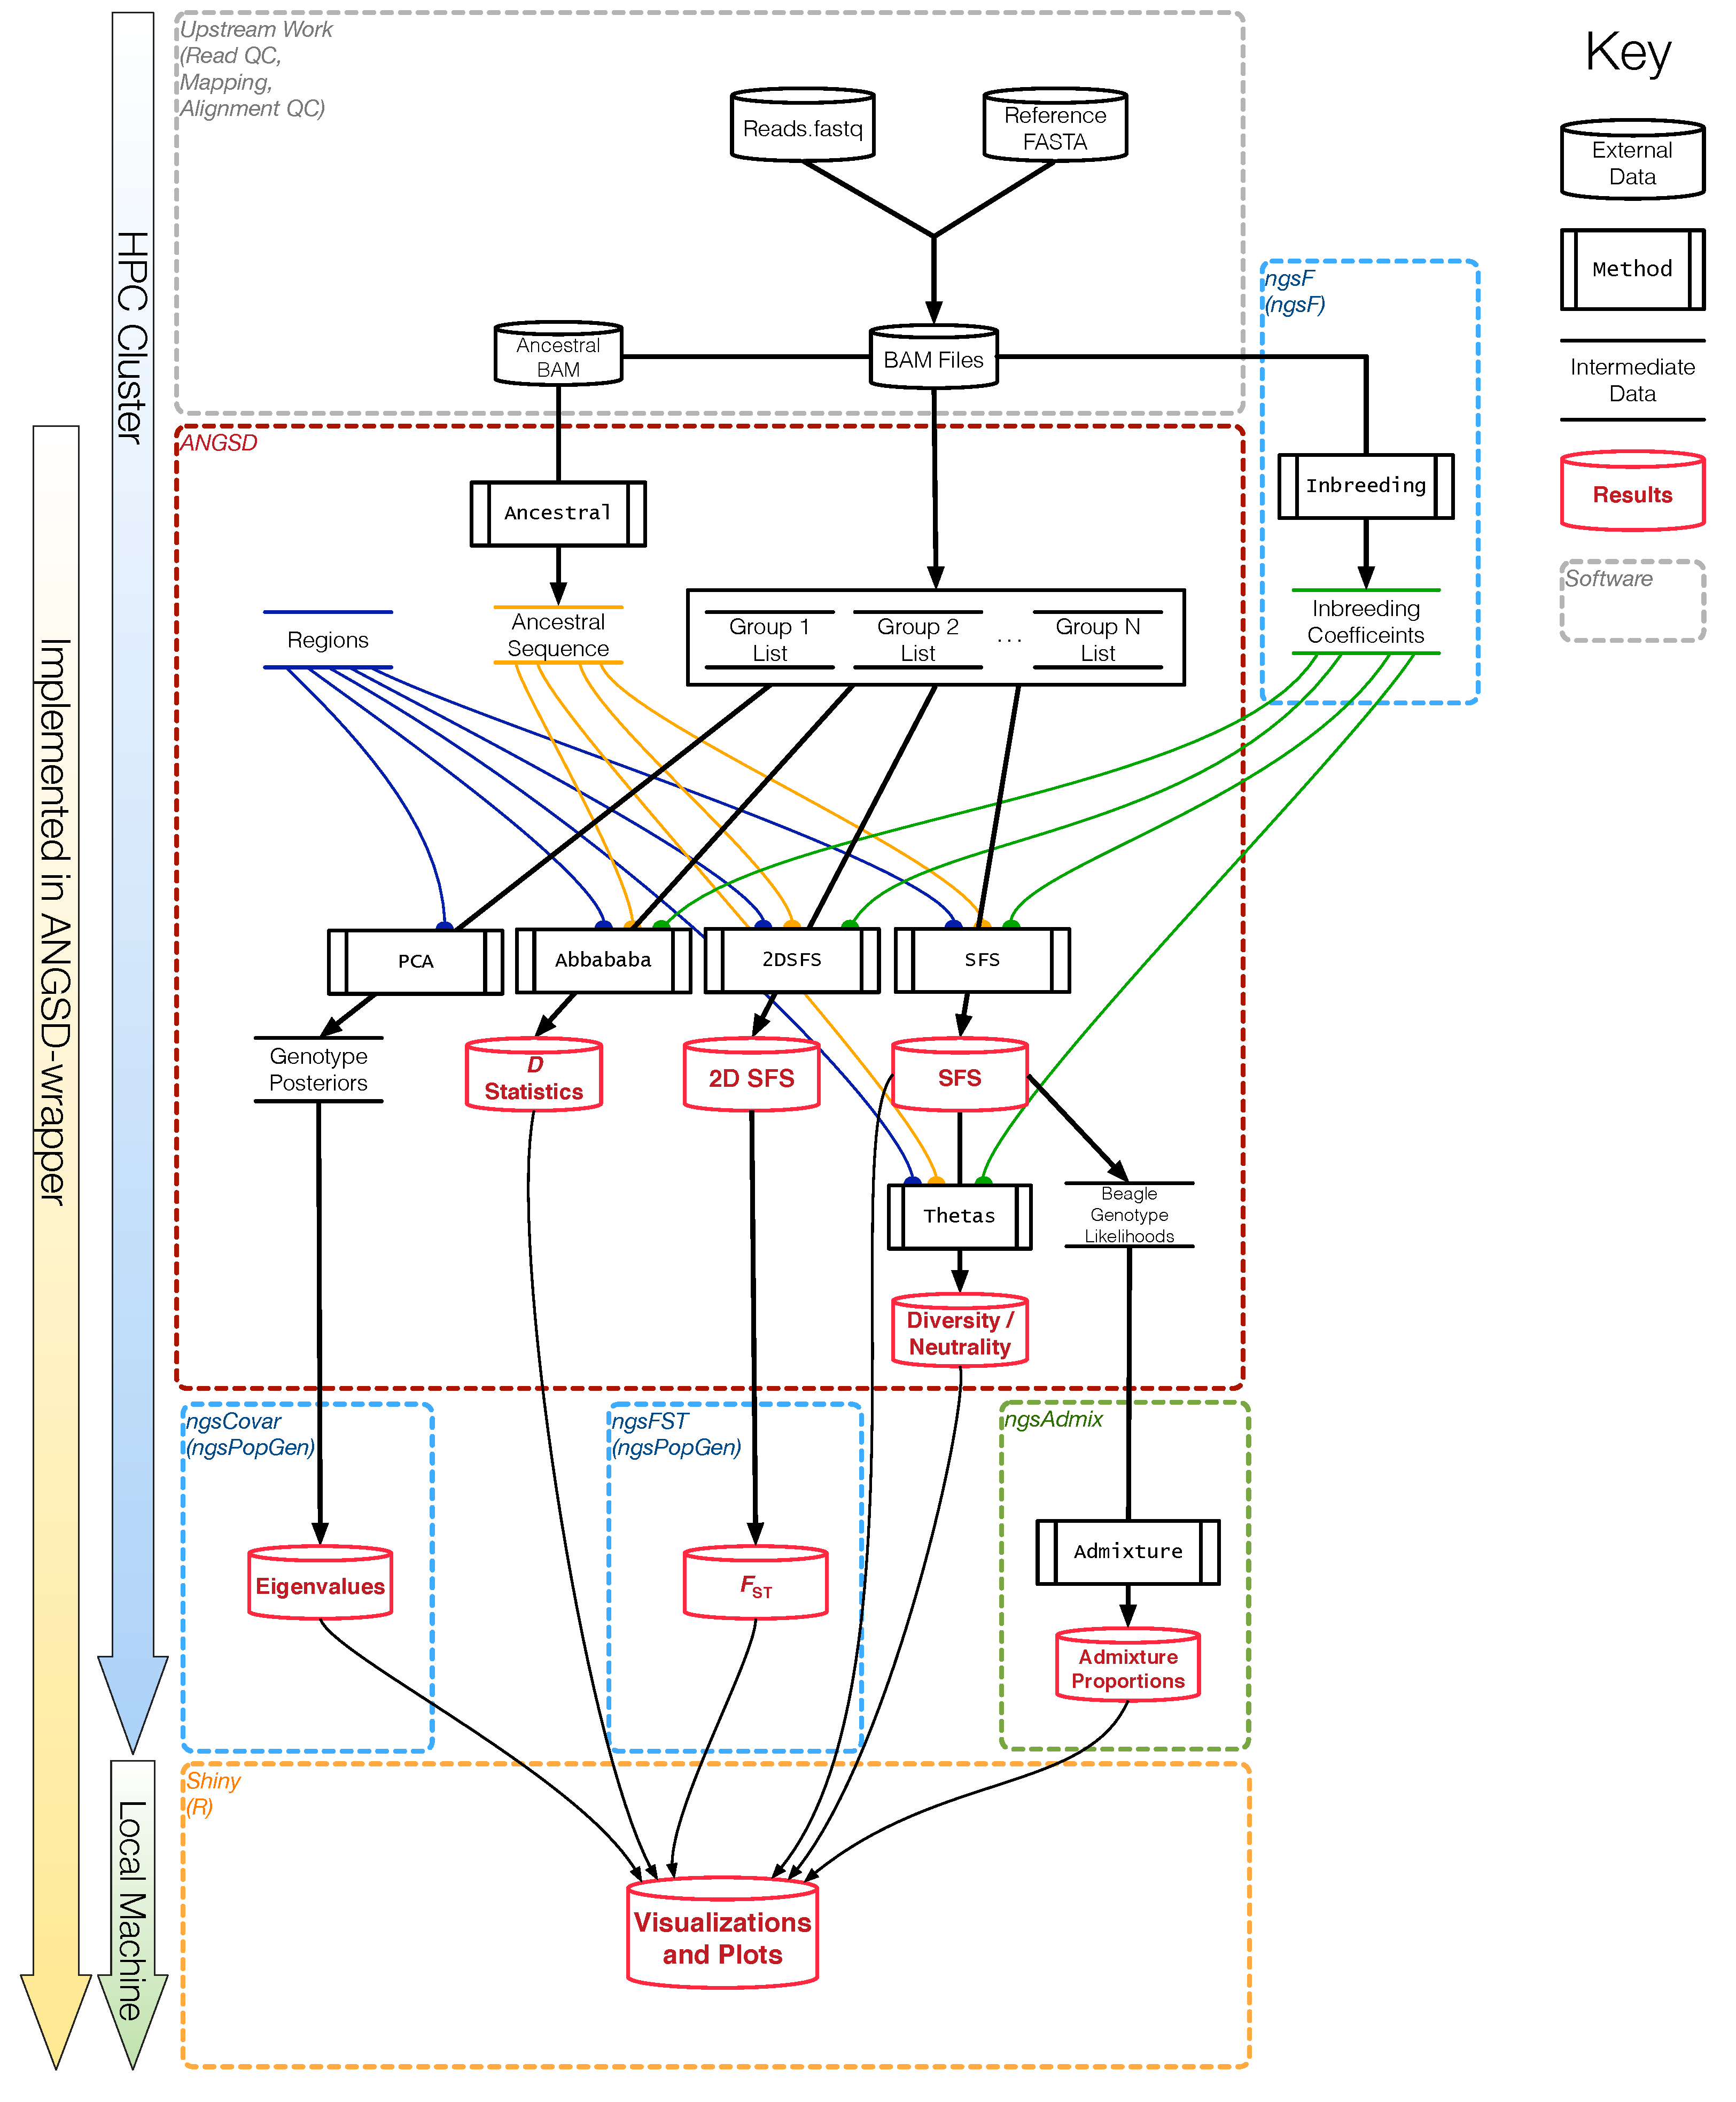
\includegraphics[width=\linewidth]{figures/Big_Workflow_newAW.pdf}
\label{fig:supp2}
\end{figure}

\begin{figure}
\centering
\caption{Admixture analysis for K=2 (top), K=3 (middle), and K=4 (bottom).}
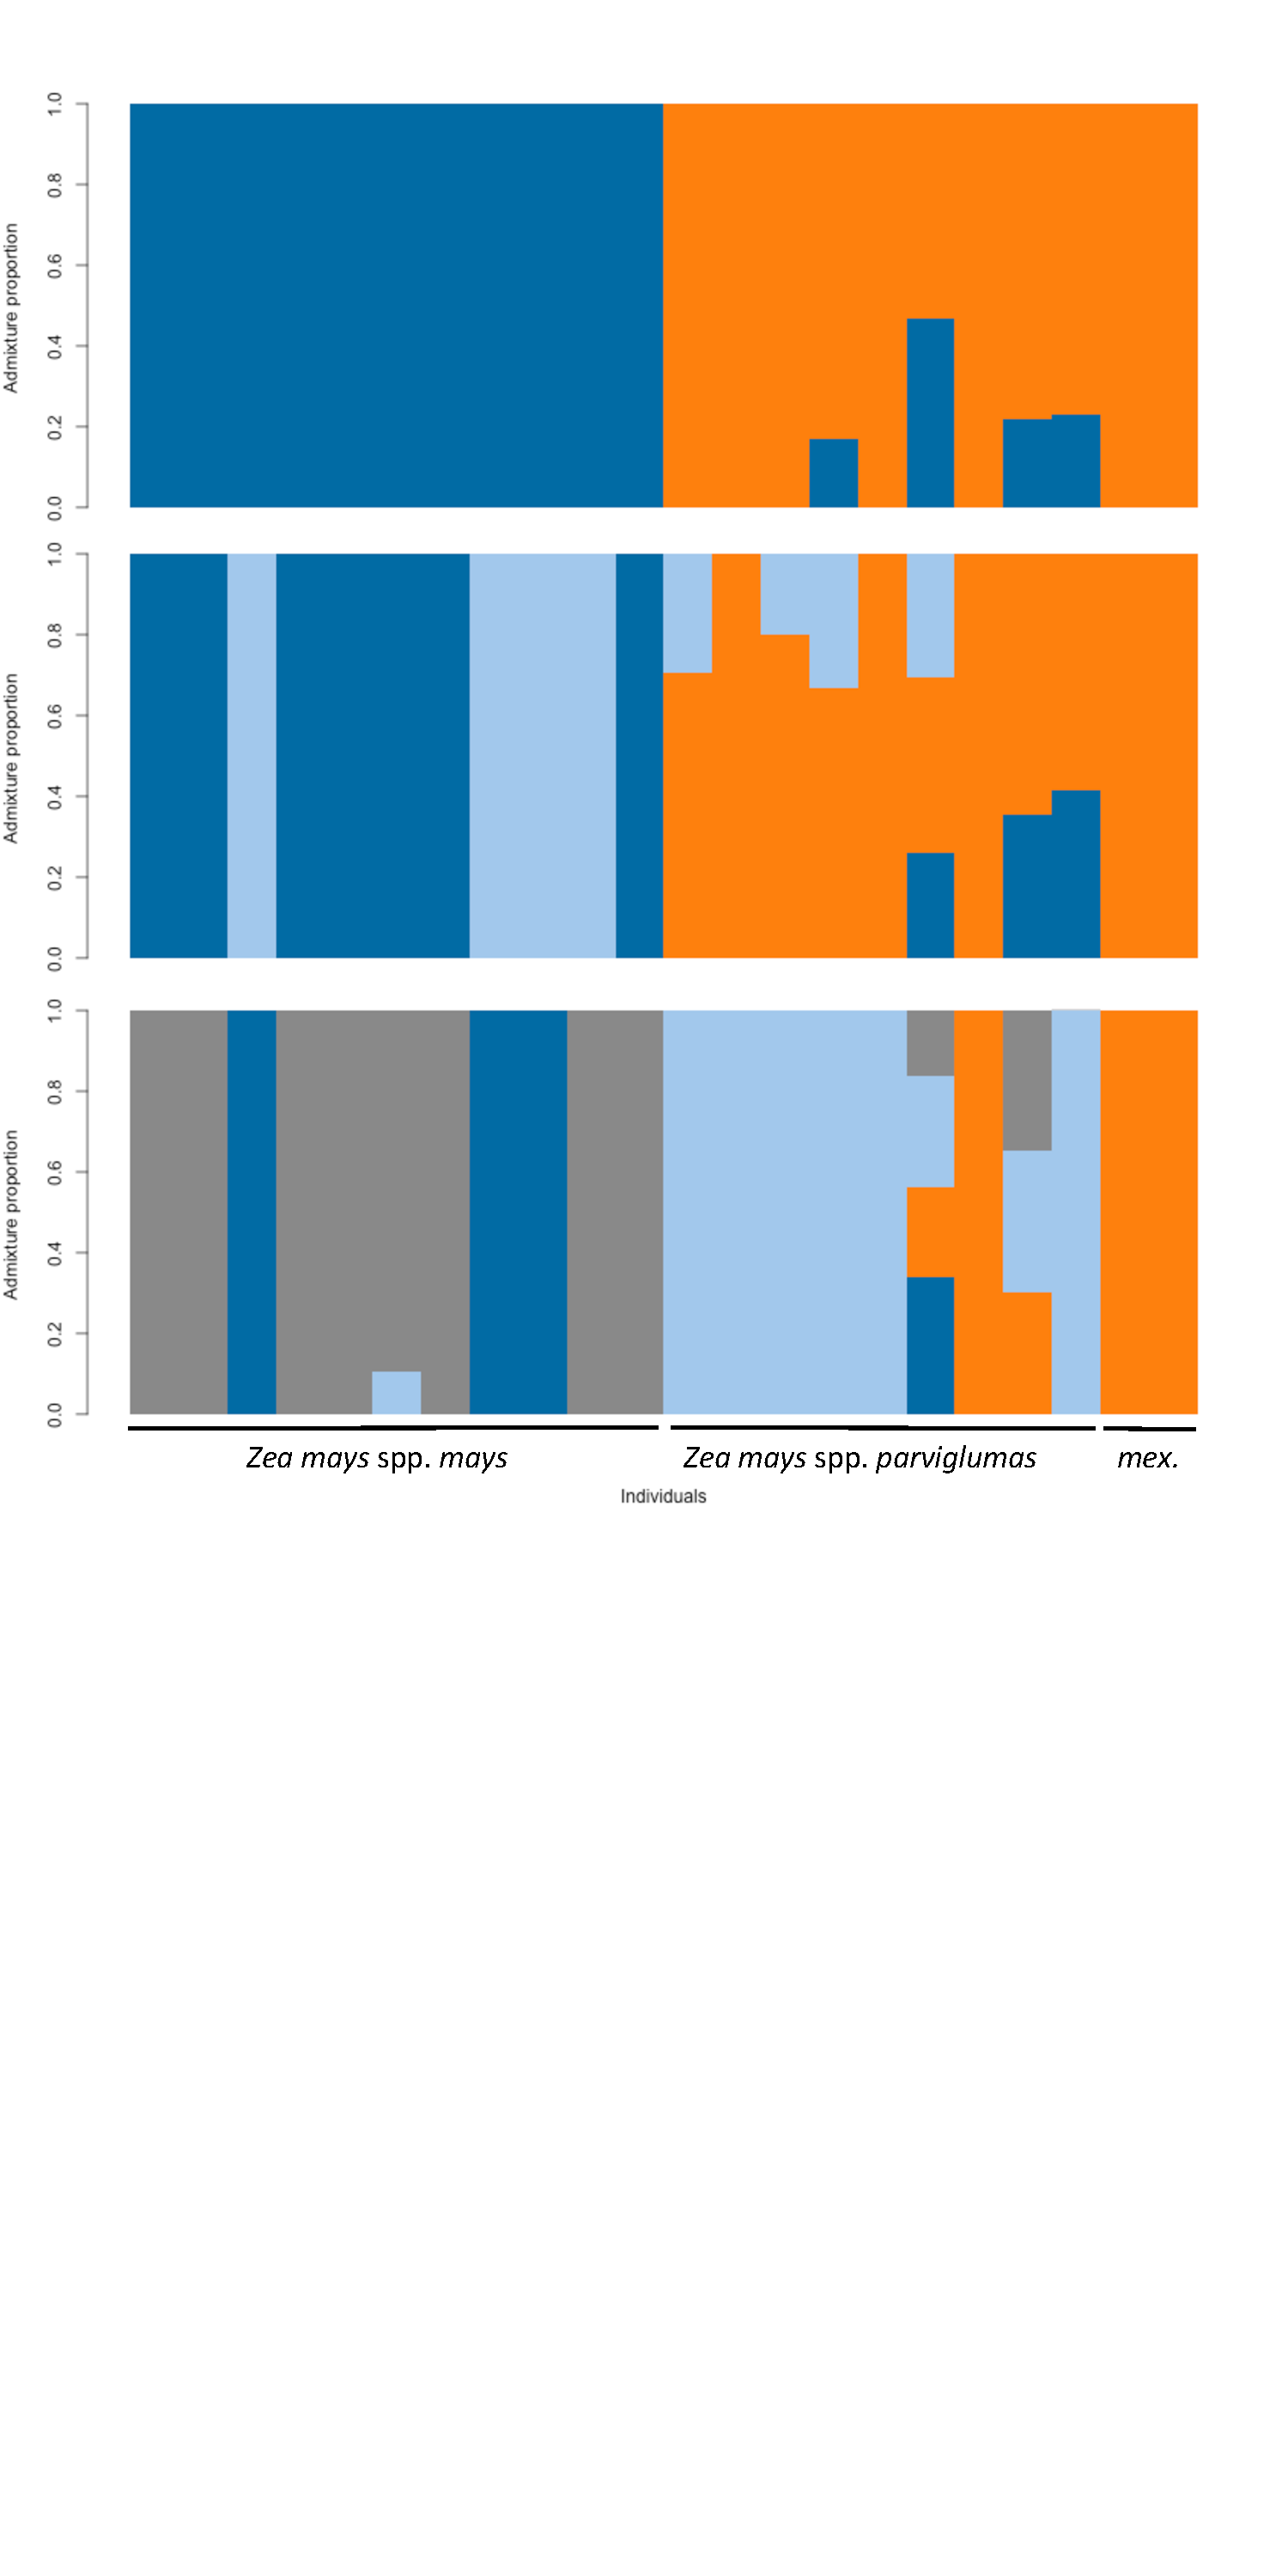
\includegraphics[width=\linewidth]{figures/admixture.pdf}
\label{fig:suppadmix}
\end{figure}

\begin{figure}
\centering
\caption{\fst values plotted against base pair position on chromosome 10 of maize. \fst is calculated between the maize and teosinte samples.}
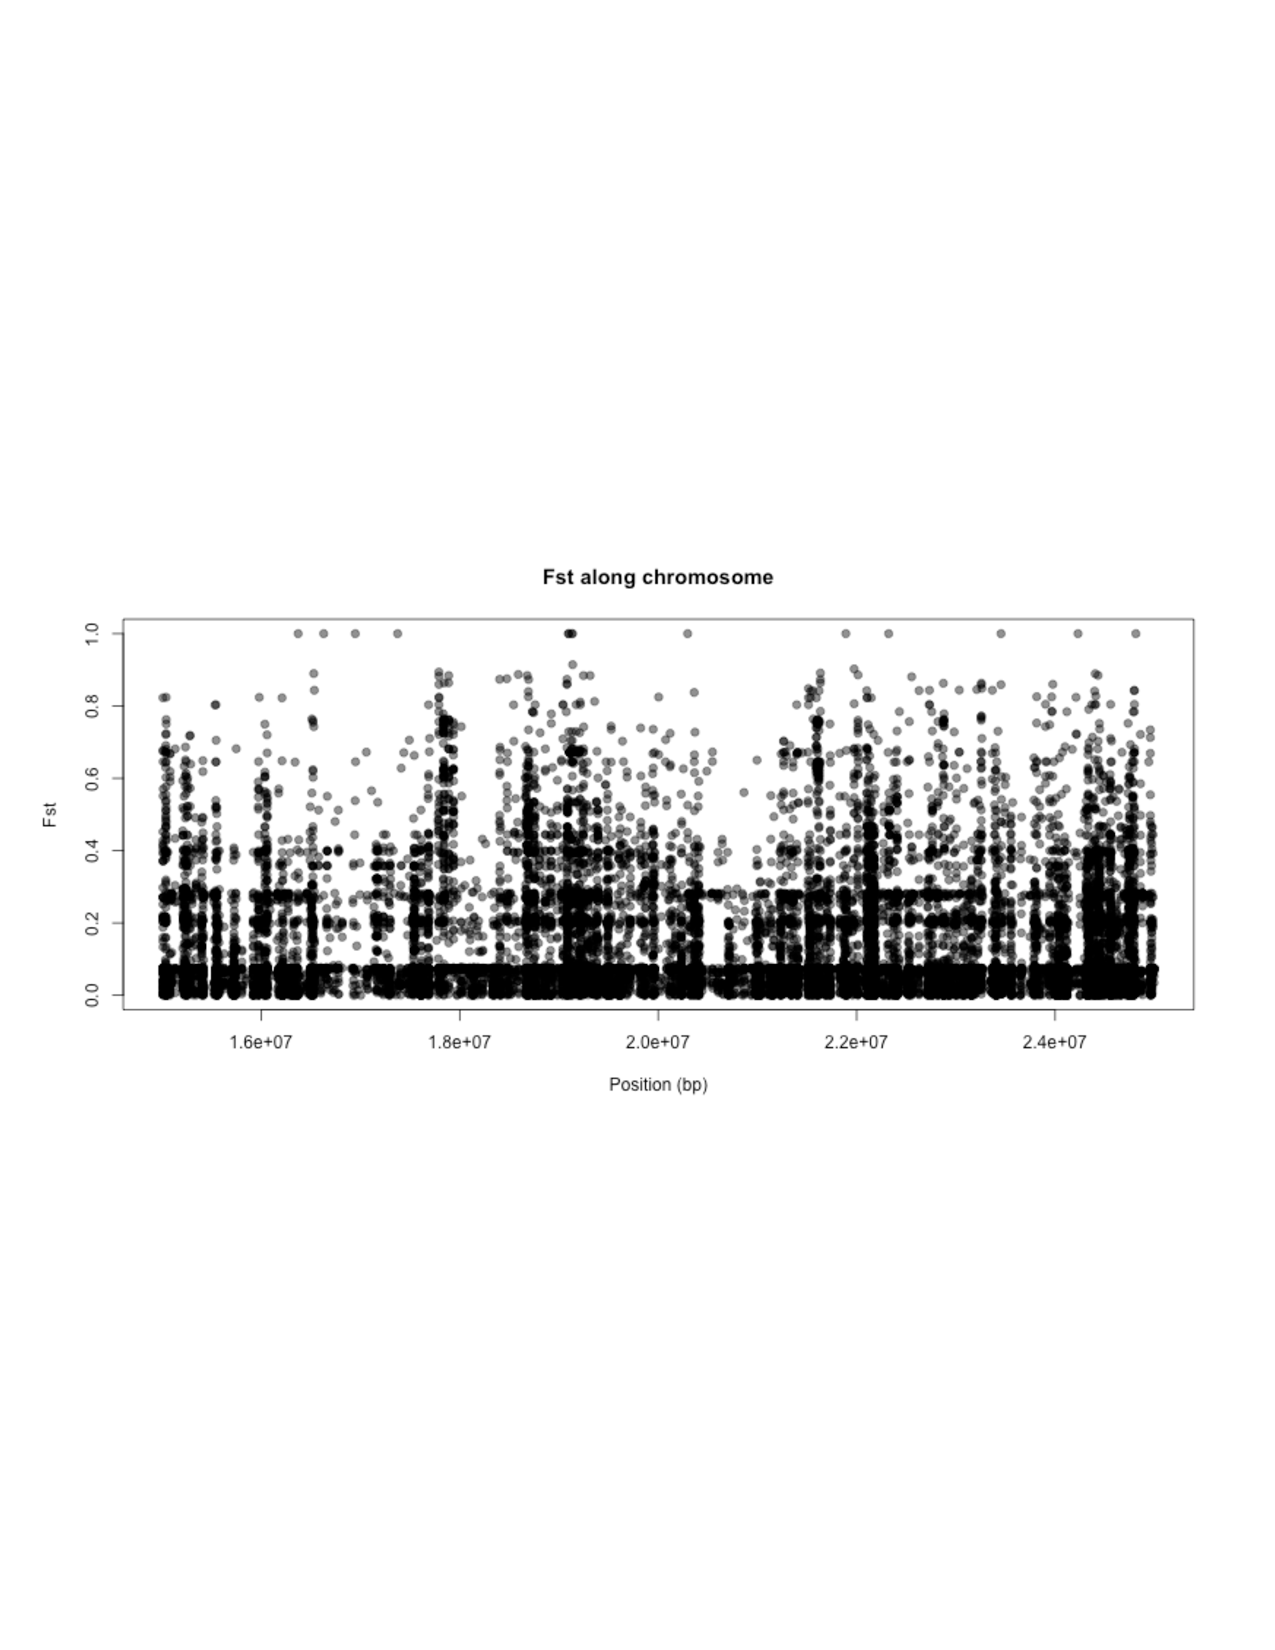
\includegraphics[width=\linewidth]{figures/supp3.pdf}
\label{fig:suppfst}
\end{figure}

\begin{table}
\begin{center}
	\caption{Table of samples used in analysis with mean depth over the region 15000000-25000000 on chromosome 10.}
	\begin{tabular} { | p{5cm} | p{5cm} | p{5cm} | }
	\hline
	\textbf{Sample} & \textbf{Mean Depth} & \textbf{Species} \\ \hline
	BKN009 & 7.00194 & {\it Zea mays} spp. {\it mays}\\ \hline
	BKN011 & 6.9777  & {\it Zea mays} spp. {\it mays}\\ \hline
	BKN014 & 6.78829 & {\it Zea mays} spp. {\it mays} \\ \hline
	BKN015 & 3.739 & {\it Zea mays} spp. {\it mays} \\ \hline
	BKN019 & 3.71944 & {\it Zea mays} spp. {\it mays} \\ \hline
	BKN022 & 3.71268 & {\it Zea mays} spp. {\it mays} \\ \hline
	BKN025 & 3.53799 & {\it Zea mays} spp. {\it mays} \\ \hline
	BKN026 & 3.91798 & {\it Zea mays} spp. {\it mays} \\ \hline
	BKN027 & 7.05576 & {\it Zea mays} spp. {\it mays} \\ \hline
	BKN033 & 3.85336 & {\it Zea mays} spp. {\it mays} \\ \hline
	BKN035 & 3.74839 & {\it Zea mays} spp. {\it mays} \\ \hline
	TIL01 & 3.60133 & {\it Zea mays} spp. {\it parviglumis}\\ \hline
	TIL03 & 4.07518 & {\it Zea mays} spp. {\it parviglumis} \\ \hline
	TIL04 & 6.09163 & {\it Zea mays} spp. {\it parviglumis} \\ \hline
	TIL07 & 5.11419 & {\it Zea mays} spp. {\it parviglumis} \\ \hline
	TIL09 & 5.29004 & {\it Zea mays} spp. {\it parviglumis} \\ \hline
	TIL11 & 3.15477 & {\it Zea mays} spp. {\it parviglumis} \\ \hline
	TIL15 & 6.87873 & {\it Zea mays} spp. {\it parviglumis} \\ \hline
	TIL16 & 2.67186 & {\it Zea mays} spp. {\it parviglumis} \\ \hline
	TIL17 & 2.61892 & {\it Zea mays} spp. {\it parviglumis} \\ \hline
	TIL08 & 6.09453 & \textit{Zea mays} ssp. {\it mexicana} \\ \hline
	TIL25 & 13.1566 & \textit{Zea mays} ssp. {\it mexicana} \\ \hline
	TDD39103 & 8.62 & \textit{Tripsacum dactyloides} \\ \hline
	\end{tabular}
	\label{tab:samples}
	\end{center}
\end{table}


\end{document}
